% 
% Annual Cognitive Science Conference
% Sample LaTeX Paper -- Proceedings Format
% 

% Original : Ashwin Ram (ashwin@cc.gatech.edu)       04/01/1994
% Modified : Johanna Moore (jmoore@cs.pitt.edu)      03/17/1995
% Modified : David Noelle (noelle@ucsd.edu)          03/15/1996
% Modified : Pat Langley (langley@cs.stanford.edu)   01/26/1997
% Latex2e corrections by Ramin Charles Nakisa        01/28/1997 
% Modified : Tina Eliassi-Rad (eliassi@cs.wisc.edu)  01/31/1998
% Modified : Trisha Yannuzzi (trisha@ircs.upenn.edu) 12/28/1999 (in process)
% Modified : Mary Ellen Foster (M.E.Foster@ed.ac.uk) 12/11/2000
% Modified : Ken Forbus                              01/23/2004
% Modified : Eli M. Silk (esilk@pitt.edu)            05/24/2005
% Modified: Niels Taatgen (taatgen@cmu.edu) 10/24/2006

%% Change ``a4paper'' in the following line to ``letterpaper'' if you are
%% producing a letter-format document.

\documentclass[10pt,letterpaper]{article}

% uncomment below to put in cogsci format
%\usepackage{cogsci}

\usepackage{pslatex}
\usepackage{apacite}
\usepackage{amsmath}
\usepackage{graphicx}
\usepackage{color}
\usepackage{amssymb}

\usepackage{algorithmic}
\usepackage{algorithm}
\usepackage{amsthm}
\usepackage{float}
\usepackage{mathrsfs}
\usepackage{fullpage}


\newcommand{\footnoteremember}[2]{
\footnote{#2}
\newcounter{#1}
\setcounter{#1}{\value{footnote}}
}
\newcommand{\footnoterecall}[1]{
\footnotemark[\value{#1}]
}


%%%%%%%%%%%%%%%%%%%%%%%%%%%%%%%%%%%%%%%%%%%%%%%%%%%%%%%%%%%%%%%%%%%%%%
% title
%%%%%%%%%%%%%%%%%%%%%%%%%%%%%%%%%%%%%%%%%%%%%%%%%%%%%%%%%%%%%%%%%%%%%%
\title{{\bf VS265 Final Project}\\Exemplar storage in associative memory systems}
 
%%%%%%%%%%%%%%%%%%%%%%%%%%%%%%%%%%%%%%%%%%%%%%%%%%%%%%%%%%%%%%%%%%%%%%
% authors
%%%%%%%%%%%%%%%%%%%%%%%%%%%%%%%%%%%%%%%%%%%%%%%%%%%%%%%%%%%%%%%%%%%%%%
\author{{\large \bf Joshua T. Abbott (joshua.abbott@berkeley.edu)\footnoteremember{myfootnote}{The authors contributed equally to this work.}} \\
 {\large \bf Jessica B. Hamrick (jhamrick@berkeley.edu)\footnoterecall{myfootnote}} \\
% {\large \bf Thomas L. Griffiths (tom\_griffiths@berkeley.edu)} \\
  Department of Psychology, University of California, Berkeley, CA 94720 USA}

\date{}

\begin{document}

\maketitle

%%%%%%%%%%%%%%%%%%%%%%%%%%%%%%%%%%%%%%%%%%%%%%%%%%%%%%%%%%%%%%%%%%%%%%
% abstract
%%%%%%%%%%%%%%%%%%%%%%%%%%%%%%%%%%%%%%%%%%%%%%%%%%%%%%%%%%%%%%%%%%%%%%
\begin{abstract}
We explore the storage of exemplars in associative memory systems as an initial investigation into neural implementations of psychological processes. We outline a recent proposal that probabilistic models of cognition accounting for human behavior at a computational level of analysis can be approximated by existing psychological process models accounting for human behavior at an algorithmic level of analysis, namely, \textit{exemplar models}. Given this motivation, the main contribution of this paper consists of analyzing the dynamics and storage capabilities of two associative models of memory: a Hopfield network, and a Sparse Distributed Memory (SDM) system. We then describe how the mechanics of SDMs can be interpreted probabilistically as a Monte Carlo method called Importance Sampling. We conclude with future directions of this research. 

% \textbf{Keywords:} 
% Sparse Distributed Memory systems, Bayesian inference, Exemplar model, Rational Process Model, Importance Sampling.
\end{abstract}

%%%%%%%%%%%%%%%%%%%%%%%%%%%%%%%%%%%%%%%%%%%%%%%%%%%%%%%%%%%%%%%%%%%%%%
% introduction
%%%%%%%%%%%%%%%%%%%%%%%%%%%%%%%%%%%%%%%%%%%%%%%%%%%%%%%%%%%%%%%%%%%%%%
\section{Introduction}

% something broad about prob models of cognition 
\cite{griffiths2010probabilistic,tenenbaum2011grow}

% something about issues with prob models
\cite{kahneman1972subjective,gigerenzer2000simple}

% something about marrs levels and that approach
\cite{marr82,anderson90}

% something about addressing these issues with RPM and bridging levels
\cite{sanborn2010rational,griffiths2012bridging}

% in particular we look at exemplar model approx
\cite{Shi2010}

%%%%%%%%%%%%%%%%%%%%%%%%%%%%%%%%%%%%%%%%%%%%%%%%%%%%%%%%%%
% subsection - exemplar models / IS for Bayes 
%%%%%%%%%%%%%%%%%%%%%%%%%%%%%%%%%%%%%%%%%%%%%%%%%%%%%%%%%%
\subsection{Exemplar models and Bayesian inference}

% maybe start with a simple example of exemplar models like Lei does.. 

% what is an exemplar model
% In an \textit{exemplar model} model of memory, people store individual instances of observations in memory (as an \textit{exemplar}) and evaluate new observations by activating these stored exemplars as a function of their similarity to this novel event \cite{medin1978context,nosofsky1986attention}. More formally, let $X^{*} = \{ x^{*}_{1}, x^{*}_{2}, \ldots, x^{*}_{n} \}$ represent a set of $n$ stored exemplars, and define $s(x,x^{*})$ to be a similarity function measuring the distance between an observation $x$ and a stored exemplar $x^{*}$. 

% -- i dont know if i like the above, i'm too tired..

% something about an identification task

\begin{equation}
	p_{r}(x^{*}_{i}|x)=\frac{s(x,x^{*}_{i})}{\sum^{n}_{j=1}s(x,x^{*}_{j})}
\end{equation}

% something about exemp models can do prob. categorization
\cite{ashby1995categorization}

% however a more general form of exemp models is

\begin{equation}
	\hat{f}(x)=\frac{\sum^{n}_{j=1}f_{j}\,s(x,x^{*}_{j})}{\sum^{n}_{j=1}s(x,x^{*}_{j})}
\end{equation}

% very brief bayes

% very brief intro to importance sampling

\cite{neal1993probabilistic,Shi2010}

%%%%%%%%%%%%%%%%%%%%%%%%%%%%%%%%%%%%%%%%%%%%%%%%%%%%%%%%%%
% subsection - previous implementations: RBFs
%%%%%%%%%%%%%%%%%%%%%%%%%%%%%%%%%%%%%%%%%%%%%%%%%%%%%%%%%%
\subsection{Neural implementations of Importance Sampling}
\cite{Shi2009}

% review Lei's components of an importance sampler

% math of RBF

% *** interesting because the RBF network is not cognitively satisfying \\
% **** all grandmother cells (and the proposed spiking neuron model was using an RBF too..) \\
% **** not robust \\


% what is an associative memory model

% something about distributed memory

% the rest of the paper explores the role of exemplars and associative memory


%%%%%%%%%%%%%%%%%%%%%%%%%%%%%%%%%%%%%%%%%%%%%%%%%%%%%%%%%%%%%%%%%%%%%%
% associative models of memory
%%%%%%%%%%%%%%%%%%%%%%%%%%%%%%%%%%%%%%%%%%%%%%%%%%%%%%%%%%%%%%%%%%%%%%
\section{Associative models of memory}



% for a full discussion, check out
\cite{Keeler1988}

%%%%%%%%%%%%%%%%%%%%%%%%%%%%%%%%%%%%%%%%%%%%%%
% subsection - Hopfield networks
%%%%%%%%%%%%%%%%%%%%%%%%%%%%%%%%%%%%%%%%%%%%%%
\subsection{Hopfield networks}
\cite{Hopfield1982}

% hopfield nets are auto-associative, meaning the whole network converges to one particular pattern given an input and does not leave this state until presented with a new input. 

% simple math of hopnet (Hebbian learning rule)
% \begin{figure}[ht!]
% \begin{center}
% 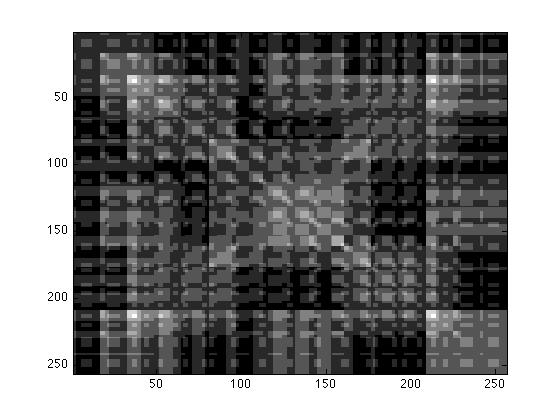
\includegraphics[width=0.8\textwidth]{./figures/hopfieldTinit.png}
% 
% \end{center}
% \caption{This is a figure.} 
% \label{sample-figure}
% \end{figure}


% known issues:
% (1) storage capacity is small fraction of number of number of neurons
% (2) can't do temporal sequences
% (3) unrealistic model of brain - requires symmetric connections
% (4) bad with correlated patterns

%%%%%%%%%%%%%%%%%%%%%%%%%%%%%%%%%%%%%%%%%%%%%%
% subsection - SDM
%%%%%%%%%%%%%%%%%%%%%%%%%%%%%%%%%%%%%%%%%%%%%%
\subsection{Sparse Distributed Memory (SDM) systems}

Sparse Distributed Memory (SDM) systems were developed by \citeA{Kanerva1988,Kanerva1993} as a mathematical model of human memory, exploiting the properties of high-dimensional representational spaces.
An SDM can function as an \textit{autoassociative}, \textit{content-addressable} memory (associates a pattern with itself) like a Hopfield network, but can additionally function as a \textit{heteroassociative} memory (associates one pattern with another), and as a \textit{sequential-access} memory (in which a temporal sequence of patterns can be stored and retrieved).

A simple way to understand how SDMs work follows from an analogue to conventional computer memory.


% \begin{figure}[t!]
% \begin{center}
% 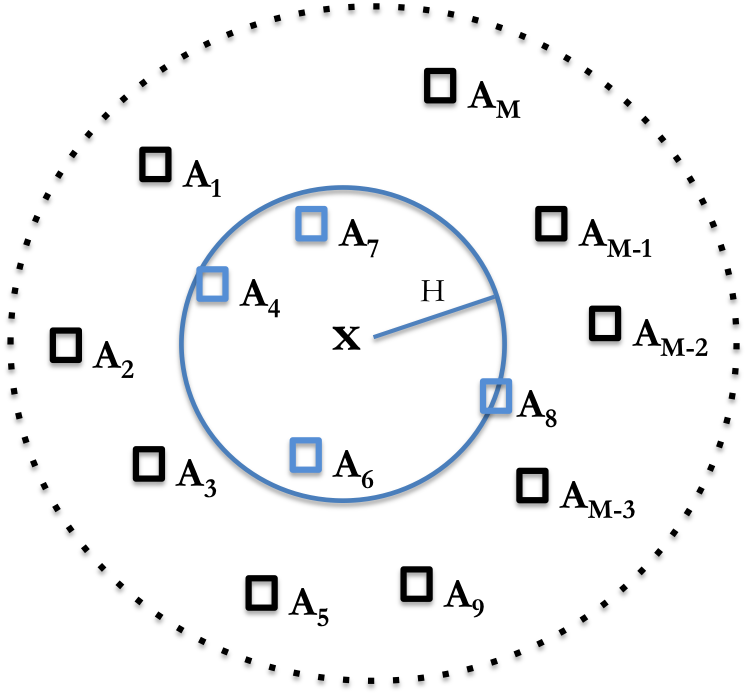
\includegraphics[width=0.5\textwidth]{./figures/sdmOperations.png}

% \end{center}
% \caption{An illustration of the basic read/write operations over SDMs. The outer dotted line represents the space of $2^{N}$ possible addresses while the squares with labels $A_{m}$ represent the $M$ sampled hard addresses used for storage. The address being requested for operation is the $X$ in the center of the blue circle of radius $H$. The hard addresses selected for operating correspond to the blue squares within the Hamming radius of $X$.} 
% \label{sdmBasics}
% \end{figure}


%%%%%%%%%%%%%%%%%%%%%%%%%%%%%%%%%%%%%%%%%%%%%%%%%%%%%%%%%%%%%%%%%%%%%%
% model evaluation
%%%%%%%%%%%%%%%%%%%%%%%%%%%%%%%%%%%%%%%%%%%%%%%%%%%%%%%%%%%%%%%%%%%%%%
\section{Exemplar storage in associative memory systems}

\begin{center}
\begin{figure*}[tb]
{
	\hfill{}
	\begin{tabular}{lclclc}
	\raisebox{2.0in}{(a)} &
		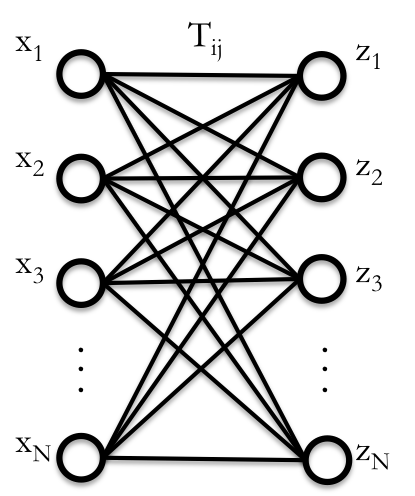
\includegraphics[width=0.24\textwidth]{./figures/hopfieldNetwork.png} &
	\raisebox{2.0in}{(b)} &
		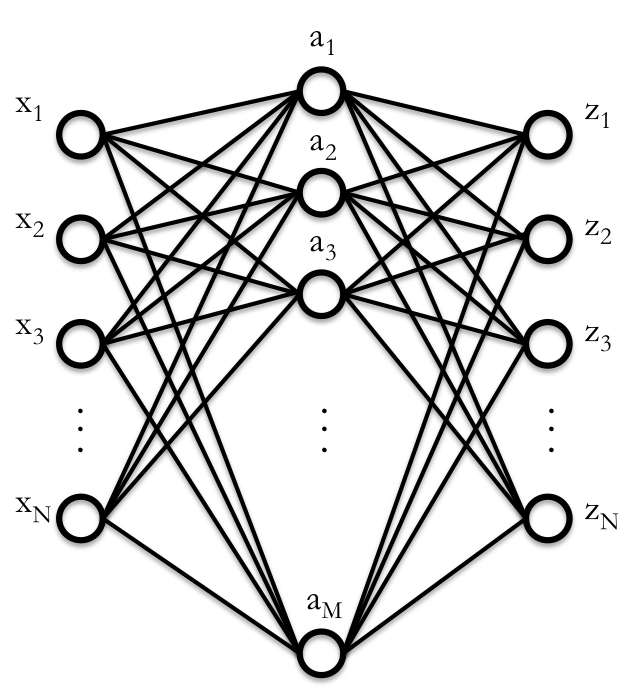
\includegraphics[width=0.27\textwidth]{./figures/sdmNetwork.png} 
	\raisebox{2.0in}{(c)} &
		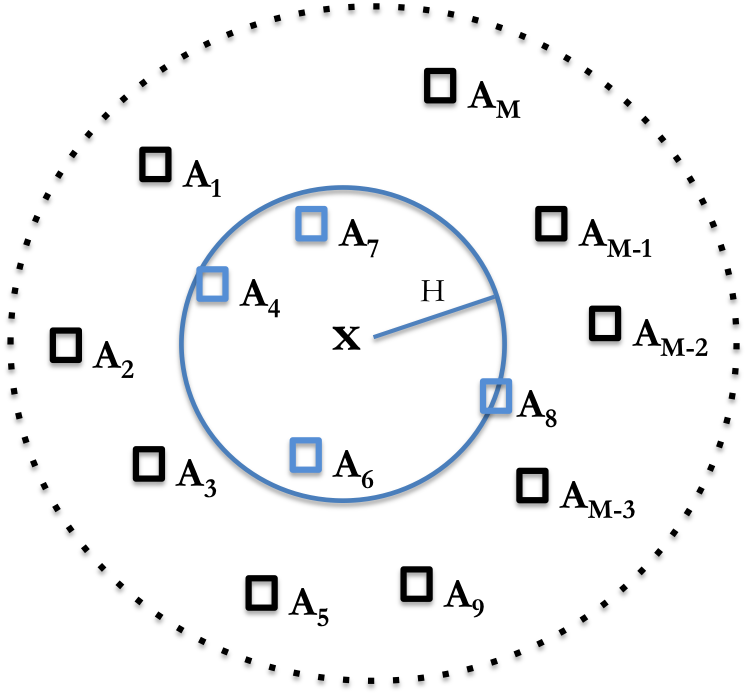
\includegraphics[width=0.29\textwidth]{./figures/sdmOperations.png} &
	\end{tabular}
}
\hfill{}
\caption{Neural network implementations of a Hopfield network (panel a) and an SDM (panel b).}
\label{neuralNets}
\end{figure*}
\end{center}

\noindent** Parameters \\
*** size of address space (think this compares to number of hidden units in others) \\
*** \# exemplars \\
*** \% bits corrupt \\

%%%%%%%%%%%%%%%%%%%%%%%%%%%%%%%%
% subsection - capacity
%%%%%%%%%%%%%%%%%%%%%%%%%%%%%%%%
\subsection{Storage Capacity}
** retrieval using corrupted and uncorrupted inputs \\


\begin{center}
\begin{figure*}[ht!]
{
	\hfill{}
	\begin{tabular}{lclc}
	\raisebox{3.75in}{(a)} &
		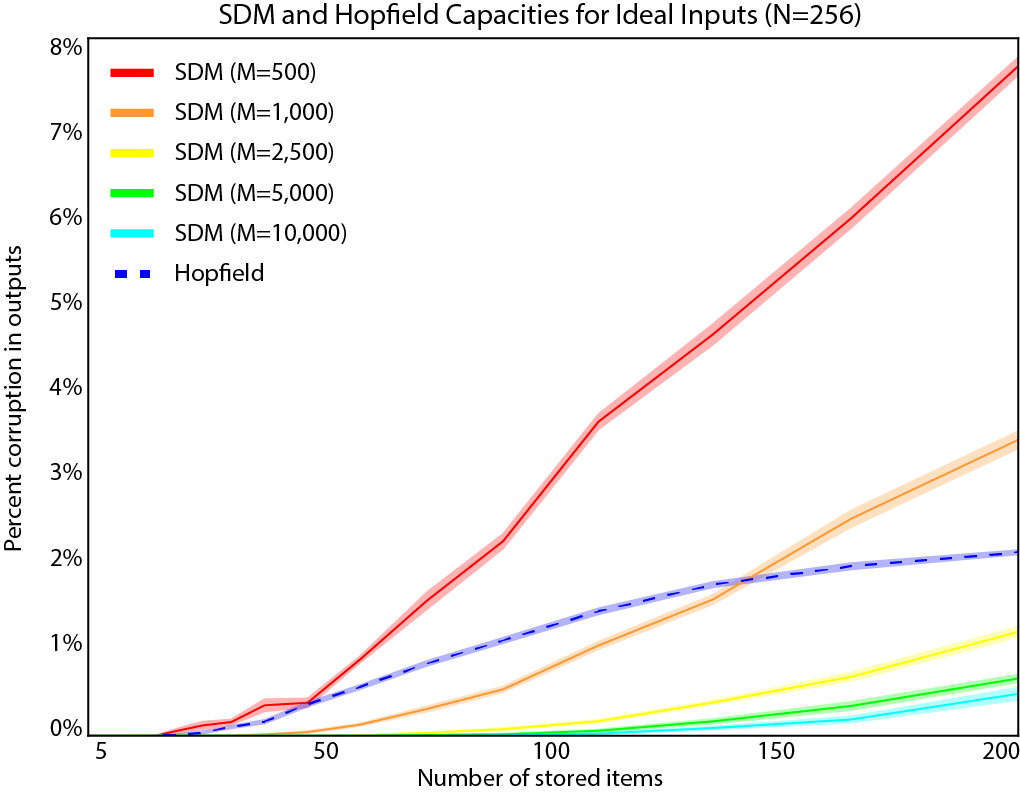
\includegraphics[width=0.4\textwidth]{./figures/capacity-edit.png}
	\raisebox{3.2in}{(b)} &
		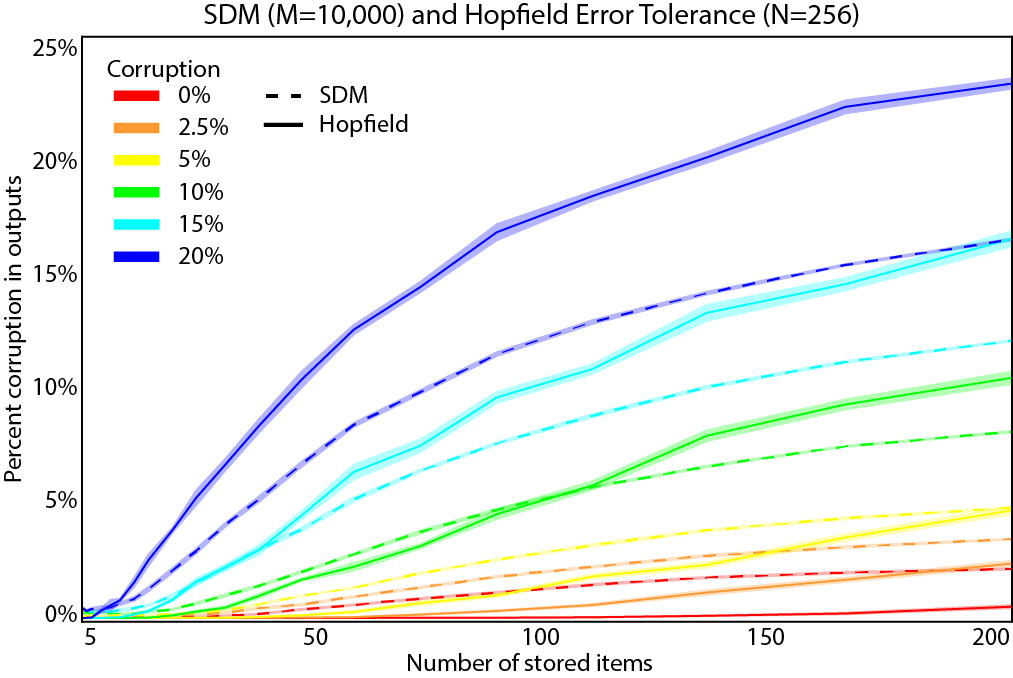
\includegraphics[width=0.4\textwidth]{./figures/tolerance-edit.png} 
	\end{tabular}
}
\hfill{}
\caption{SDM and Hopfield network capacities (panel a) and error tolerances (panel b).}
\label{capacityAndErrorTolerance}
\end{figure*}
\end{center}


%%%%%%%%%%%%%%%%%%%%%%%%%%%%%%%%
% subsection - prototypes
%%%%%%%%%%%%%%%%%%%%%%%%%%%%%%%%
\subsection{Prototype Retrieval}

% what happens when we try to store the noisy circles in an hopnet, does it converge to a prototype as well?


\begin{center}
\begin{figure*}[ht!]
{
	\hfill{}
	\begin{tabular}{ l l l c}
	\raisebox{2.5in}{(a)} &
		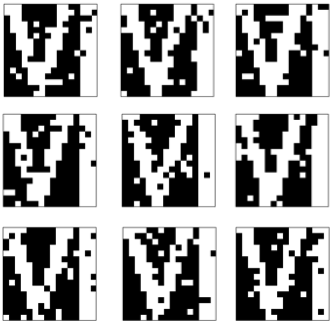
\includegraphics[width=0.43\textwidth]{./figures/exemplars.png} &
	\raisebox{2.5in}{(b)} &
		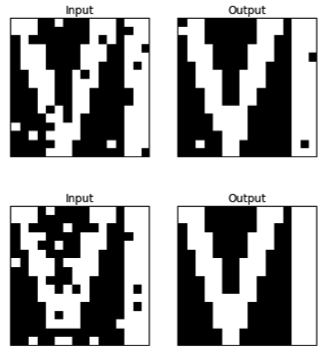
\includegraphics[width=0.4\textwidth]{./figures/prototypeResults.png} \\
	%	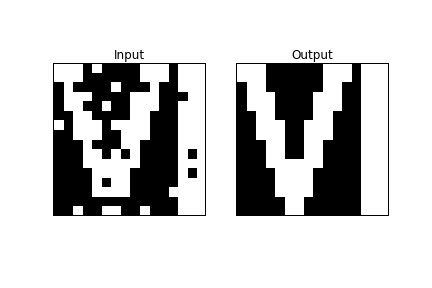
\includegraphics[width=0.4\textwidth]{./figures/vi_sdm.png} 
	\end{tabular}
}
\hfill{}
\caption{(a) Nine noisy exemplars stored in both SDM and Hopfield models. (b) The retrieval results for the Hopfield network (top) and SDM network (bottom) when queried with a noisy word.}
\label{prototypes}
\end{figure*}
\end{center}


% - even if it does, it can't really store much else without really messing things up due to its capacity, where in SDM it's just a tiny fraction of the space of things - ie, does storing noisy faces, numbers, circles, AND sequences do anything to the retrieval of the prototype?

\begin{figure}[ht!]
\begin{center}
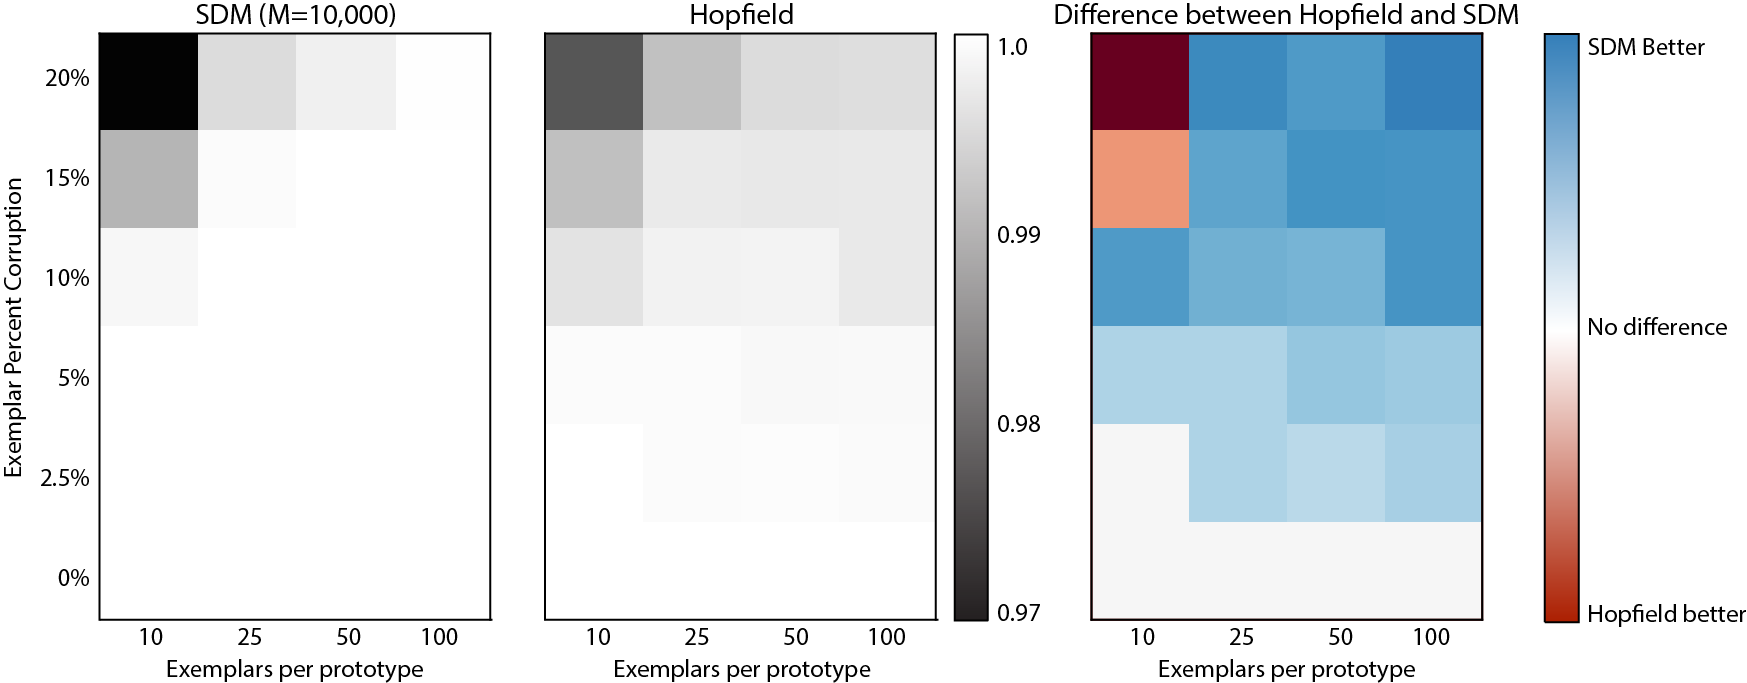
\includegraphics[width=0.95\textwidth]{./figures/prototype-edit.png}

\end{center}
\caption{This is a figure.} 
\label{sample-figure}
\end{figure}


%%%%%%%%%%%%%%%%%%%%%%%%%%%%%
% subsection - sequences
%%%%%%%%%%%%%%%%%%%%%%%%%%%%%
\subsection{Sequence Storage}

% just to show off here since the hopnet can't at all - but maybe we should make a comment about recurrent nets (JUST a comment) ?
\begin{center}
\begin{figure*}[ht!]
{
	\hfill{}
	\begin{tabular}{ l c }
	\raisebox{4.1in}{(a)} &
		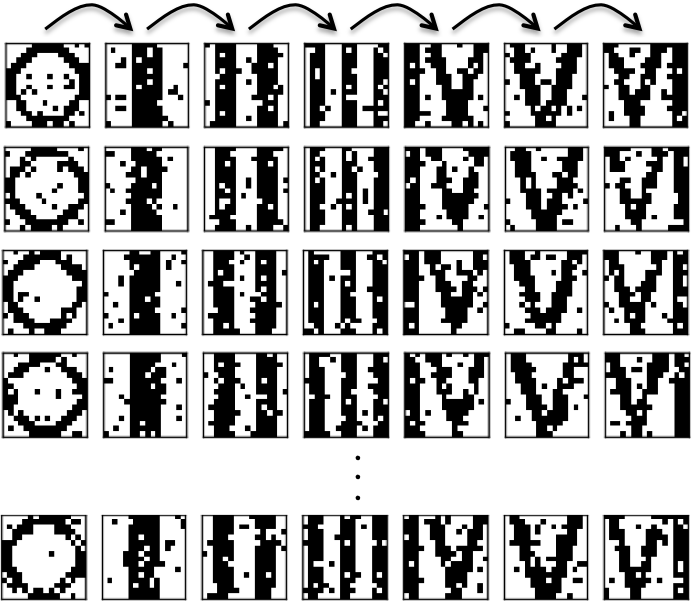
\includegraphics[width=0.8\textwidth]{./figures/exemplarStoredSequences.png} \vspace{25bp} 
		\\
	\raisebox{.6in}{(b)} &
		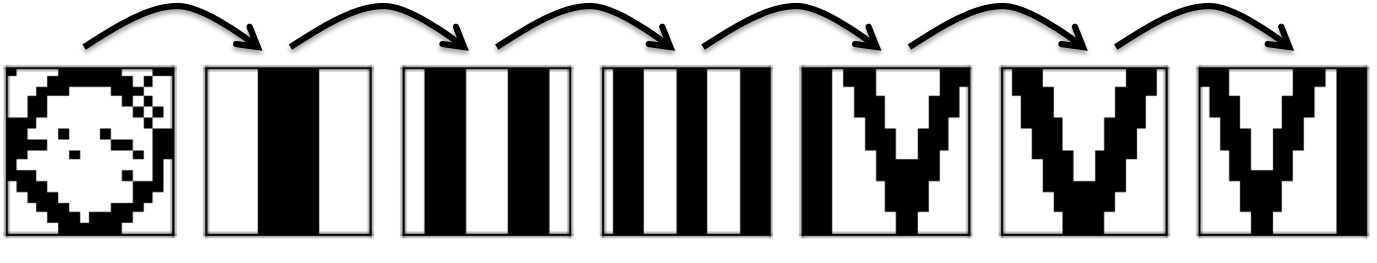
\includegraphics[width=0.8\textwidth]{./figures/prototypeRetrievedSequence.png} 
	\end{tabular}
}
\hfill{}
\caption{(a) Exemplars of noisy sequences stored in SDM memory. (b) Retrieval of prototypical sequence in SDM from a noisy word.}
\label{sequences}
\end{figure*}
\end{center}



%%%%%%%%%%%%%%%%%%%%%%%%%
% subsection - discussion
%%%%%%%%%%%%%%%%%%%%%%%%%
\subsection{Discussion}

% wrap up results from evaluations

% ** SDM is the best \\
% only the only model that is both robust to noise/storage capacity and
% sophisticated enough to behave in various ways 

** difference between addresses and data \\
% - address/data difference is called heteroassociative memory (associate one pattern with another - i think...)



%%%%%%%%%%%%%%%%%%%%%%%%%%%%%%%%%%%%%%%%%%%%%%%%%%%%%%%%%%%%%%%%%%%%%%
% future directions
%%%%%%%%%%%%%%%%%%%%%%%%%%%%%%%%%%%%%%%%%%%%%%%%%%%%%%%%%%%%%%%%%%%%%%
\section{Probabilistic interpretations of SDMs}

% *** probabilistic interpretations \cite{Anderson1989}\\
% *** figure out the encoding for importance sampling \\
% *** how close does it have to be to the delta function? \\

Exemplar models have more potential than uniformly storing data and
recovering its mean. \citeA{Shi2010} demonstrated that exemplar models
can be used to implement \textit{importance sampling}, a Monte Carlo
method of approximating Bayesian inference.  Can SDMs be used to
implement importance sampling? Previous work has formalized a
probabilistic interpretation of SDMs \cite{Anderson1989}, thus
suggesting that it should be possible to adjust that formalization to
specifically encompass exemplar-based approximate inference. Here, we
extend the idea of using exemplar models for importance sampling in
the context of SDMs.

\subsection{Overview}

In general, our goal is to use SDMs to recover the expectation of some
function $f(x^*)$. However, we cannot directly observe $x^*$; instead,
we have observations $x$. Importance sampling provides a way for us to
infer the value of $x^*$ given our observations, and therefore compute
$y$. This is given by Eq. 12 in \citeA{Shi2010}:
\begin{equation}
E[f(x^*)|x]\approx \frac{\sum_j f(x_j^*)\Pr(x|x_j^*)}{\sum_j \Pr(x|x_j^*)}
\end{equation}

To translate this into the context of a SDM, let $x^*$ be the
uncorrupted target address at which we want to read or write a value
$y$. If $x$ is a corrupted version of $x^*$, then we wish to choose
some addresses $a_j$ given $x$ such that reading and writing to those
addresses approximate reading and writing $(x^*,y)$. This is
equivalent to computing the expectation of $f(x^*)=y$ over the
addresses $a_j$.

\subsection{Writing}

Let us define the probability of writing to address $a_j$ given an
input address $x_i^*$ as $w(a_j|x_i^*)$. In the limit, the number of
addresses increases to the point where we will always be able to write
to exactly $x_i^*$. Thus, this writing density must satisfy the
following constraint:
\begin{equation}
\lim_{M\rightarrow 2^N}w(a_j|x_i^*) = \delta(a_j=x_i^*)
\label{eq:w}
\end{equation}

After writing multiple values $(x_i^*, y)$, the value of the counter
associated with address $a_j$ will be:
\begin{equation}
C_j=\sum_i w(a_j|x_i^*)y_i
\label{eq:Cj}
\end{equation}

\subsection{Reading}

We are given an address $x$, which as before is a corrupted version of
$x^*$; the goal is to read the value stored at $x^*$. We can define
reading distribution as the likelihood that $x$ was generated from
some $a_j$:
\begin{equation}
r(x| a_j)\propto \Pr(x|x^*=a_j)
\label{eq:r}
\end{equation}

We weight the counter value $C_j$ for each $a_j$ based on the
likelihood that $a_j$ is the actual target address. The sum over these
values is:
\begin{equation}
f(x)=\sum_j C_j r(x| a_j)
\label{eq:R}
\end{equation}

% \begin{equation}
% R(x) = 
% \end{equation}

The expected value of this sum over all addresses $a$ is obtained by
substituting Eq. \ref{eq:Cj} into Eq. \ref{eq:R} and simplifying due
to linearity of expectation:
\begin{align}
\mathbb{E}_a[f(x)]&=\mathbb{E}_a\left[\sum_j\left(\sum_i w(a_j| x_i^*)y_i\right)r(x|a_j)\right]\\
&=\sum_i\ y_i\cdot E_a\left(\sum_j w(a_j| x_i^*)r(x|a_j)\right)
\end{align}

As our address space grows larger (as in Eq. \ref{eq:w}), this approaches:
\begin{align}
\lim_{M\rightarrow 2^N} \mathbb{E}_a[f(x)]&=\sum_i\ y_i \int_a \delta(a-x_i^*)\Pr(x|x^*=a)\ \mathrm{d}a\\
&= \sum_i\ y_i\Pr(x|x_i*)
\end{align}

Thus, in the limit, the expected value that we read out will be:
\begin{equation}
\mathbb{E}[y|x]\propto \sum_i\ y_i\Pr(x|x_i^*)
\end{equation}

\subsection{Empirical comparison}

To verify this formulation of the SDM as an importance sampler, we 


%%%%%%%%%%%%%%%%%%%%%%%%%%%%%%%%%%%%%%%%%%%%%%%%%%%%%%%%%%%%%%%%%%%%%%
%  conclusions
%%%%%%%%%%%%%%%%%%%%%%%%%%%%%%%%%%%%%%%%%%%%%%%%%%%%%%%%%%%%%%%%%%%%%%
\section{Conclusions}



% \begin{table}[!ht]
% \begin{center} 
% \caption{Sample table title.} 
% \label{sample-table} 
% \vskip 0.12in
% \begin{tabular}{ll} 
% \hline
% Error type    &  Example \\
% \hline
% Take smaller        &   63 - 44 = 21 \\
% Always borrow~~~~   &   96 - 42 = 34 \\
% 0 - N = N           &   70 - 47 = 37 \\
% 0 - N = 0           &   70 - 47 = 30 \\
% \hline
% \end{tabular} 
% \end{center} 
% \end{table}

% \begin{figure}[ht]
% \begin{center}
% \fbox{CoGNiTiVe ScIeNcE}
% \end{center}
% \caption{This is a figure.} 
% \label{sample-figure}
% \end{figure}




%%%%%%%%%%%%%%%%%%%%%%%%%%%%%%%%%%%%%%%%%%%%%%%%%%%%%%%%%%%%%%%%%%%%%%
% bibliography
%%%%%%%%%%%%%%%%%%%%%%%%%%%%%%%%%%%%%%%%%%%%%%%%%%%%%%%%%%%%%%%%%%%%%%
\newpage
\bibliographystyle{apacite}

\setlength{\bibleftmargin}{.125in}
\setlength{\bibindent}{-\bibleftmargin}

\bibliography{classProject}


%%%%%%%%%%%%%%%%%%%%%%%%%%%%%%%%%%%%%%%%%%%%%%%%%%%%%%%%%%%%%%%%%%%%%%
% appendix (code)
%%%%%%%%%%%%%%%%%%%%%%%%%%%%%%%%%%%%%%%%%%%%%%%%%%%%%%%%%%%%%%%%%%%%%%
\newpage
\appendix

\section{Project Code}
This is where we have the code.


\end{document}
